\chapter{エントロピーとエネルギーから見た温度}

\lectureoverview{温度は、まず人間の温度計の単位を微視的なエネルギーの単位へ変換するものとして現れる。熱力学的エントロピーから無次元の統計的エントロピーへの対応する変換を行った後、我々は平衡状態を1つのパラメータで表される確率分布の族によって記述する。その導関数\(dE/dS\)が温度を定義し、最初の2つの法則は、なぜ温度差がエネルギーの流れの向きを決めるのかを示している。}

\section{換算係数と人間の単位}

物理学の多くの定数は換算係数である。光速は距離を時間に変換する：
\begin{equation}
 t=\frac{x}{c}.
\end{equation}
距離と時間が整合した単位で測られるならば、\(c=1\)と置いてよい。物理的効果は何も消えず、2種類の測定が単に1つの共通の尺度に置かれただけである。

ボルツマン定数も同じ性格をもつ。それは人間の尺度の温度計で読み取られる温度をエネルギーに変換する。\emph{人間の尺度の}という形容詞は重要である。そのような単位は、巨視的な計器が生成し分解できるという理由で選ばれており、微視的な力学がそれらを特別に選び出しているからではない。

摂氏度は、標準圧力における水の凝固点と沸点の間の間隔を100等分することによって定められた。ケルビンは同じ大きさの度を用いるが、零点を絶対零度に置く。異なる物質、異なる間隔、あるいは華氏度を選べば数値は変わるが、物理は変わらない。

\begin{classroomqa}
\audiencequestion{華氏の目盛りはすでに17世紀の構築物だったのか。}
\lecturerresponse{正確な年代はここでは必要ない。要点は、そのような目盛りはすべて、人々が用意し測定できる温度を中心に設計されたということである。それらの度の大きさは微視的というより慣習的である。
\lecturetimestamp{00:01:34--00:01:50}}
\end{classroomqa}

これらの目盛りが作られた当時、熱の分子的起源は実験に利用できなかった。1度の変化は巨視的な温度計で観測できたが、1分子のエネルギーは測定できなかった。したがって、温度が根本的にはエネルギーの尺度であると誰も知る前に、温度の単位を発明するのは自然であった。

\section{なぜ温度はエネルギーの単位をもつのか}

希薄な単原子気体を考える。希薄とは、ここでの目的のためには分子間の相互作用エネルギーを無視してよいことを意味する。熱平衡においては、エネルギー等分配則により、並進運動の各二次の自由度に\(T_{\mathrm K}/2\)とボルツマン定数の積が割り当てられる。三次元空間では、\begin{equation}
 \left\langle E_{\mathrm{kin}}\right\rangle
 =\frac{3}{2}k_{\mathrm B}T_{\mathrm K}.
 \label{eq:sm2-equipartition-kelvin}
\end{equation} 係数の3は\(x\)、\(y\)、\(z\)方向の運動を数えたものである。係数の2分の1は二次の運動エネルギーに由来する。

この関係は特定の分子種に固有のものではない。平衡状態にあるヘリウムと酸素の混合物では、自由に並進するすべての粒子が同じ平均重心運動エネルギーをもつ。より重い粒子はよりゆっくり動くにもかかわらず、である。
\begin{equation}
 E_{\mathrm{kin}}=\frac{1}{2}mv^2,
\end{equation}
より、等しい特徴的エネルギーは\(v\propto m^{-1/2}\)を意味する。

同じ考えは、意図的に極端な例にまで押し進めることができる。ボウリングの球を流体中に吊るし、系全体を平衡に到達させる。そのブラウン並進自由度は、分子のそれらと同じエネルギーの尺度に支配される。球の速度は、その質量が途方もなく大きいために途方もなく小さいが、温度は速さではなくエネルギーの尺度を比較するのである。

室温では、\(T_{\mathrm K}\)はおよそ\(300\,\mathrm K\)であるが、1つの微視的自由度のエネルギーはジュールではごく小さい。したがって換算係数はごく小さい：
\begin{equation}
 k_{\mathrm B}\simeq 1.38\times10^{-23}\,
 \mathrm{J\,K^{-1}}.
 \label{eq:sm2-boltzmann-value}
\end{equation}
その大きさとアボガドロ数は偶然ではなく関係している：
\begin{equation}
 R=N_{\mathrm A}k_{\mathrm B}.
\end{equation}
気体定数\(R\)はモルを記述し、一方\(k_{\mathrm B}\)は対応する尺度を微視的な構成要素あたりで記述する。

基本公式には繰り返し組み合わせ\(k_{\mathrm B}T_{\mathrm K}\)が現れる。したがって、
\begin{equation}
 T\equiv k_{\mathrm B}T_{\mathrm K}.
 \label{eq:sm2-energy-temperature}
\end{equation}
と定義する方がすっきりしている。以後、\(T\)自体がエネルギーの単位をもち、\eqref{eq:sm2-equipartition-kelvin}は
\begin{equation}
 \left\langle E_{\mathrm{kin}}\right\rangle=\frac{3}{2}T.
 \label{eq:sm2-equipartition-natural}
\end{equation}
となる。エネルギーをジュールで測るならば、温度もジュールで測られる。エネルギーを電子ボルトで測るならば、温度も電子ボルトで測られる。温度単位と呼ばれる新たな自然の単位は存在しない。

\section{エントロピーに関する2つの規約}

同じ換算はエントロピーの側にも現れる。巨視的な熱力学は熱機関の解析から生まれた。カルノーは決定的な熱機関の推論を与え、クラウジウスは後に熱力学的エントロピーと記号\(S\)を導入した。ここで用いる記法では、その巨視的量を\(S_{\mathrm C}\)と呼ぶ。その単位はエネルギーを温度計の温度で割ったもの、たとえばジュール毎ケルビンである。

統計エントロピーは無次元である。離散分布に対して、
\begin{equation}
 S=-\sum_i p_i\log p_i.
 \label{eq:sm2-statistical-entropy}
\end{equation}
自然対数を用いると、公平な二値の選択肢のエントロピーは\(\log2\)である。底を2とする対数を用いると、同じ量は1ビットと呼ばれる。二つのエントロピーの規約は次で関係づけられる。
\begin{equation}
 S=\frac{S_{\mathrm C}}{k_{\mathrm B}},
 \qquad
 S_{\mathrm C}=k_{\mathrm B}S.
 \label{eq:sm2-entropy-conversion}
\end{equation}
\(\mathrm{J\,K^{-1}}\)で控えめな巨視的値は、膨大な数の微視的構成要素の間に分配された情報を数えるため、膨大な無次元エントロピーに対応する。

式\eqref{eq:sm2-energy-temperature}と式\eqref{eq:sm2-entropy-conversion}は、以下で用いられる規約を確立する。
\[
 [T]=[\text{energy}],
 \qquad
 [S]=1.
\]
ボルツマン定数は、これで実用的な公式から消えることができる。常に\(T\)を\(k_{\mathrm B}T_{\mathrm K}\)に、\(S\)を\(S_{\mathrm C}/k_{\mathrm B}\)に置き換えることで復元できる。

\begin{classroomqa}
\audiencequestion{因子\(3/2\)を除けば、新しい温度は単にジュールで測ったエネルギーなのか。}
\lecturerresponse{はい、ジュールが選ばれたエネルギー単位ならばそうである。ジュールはMKS単位\(\mathrm{kg\,m^2\,s^{-2}}\)である。代わりに電子ボルトや他の任意のエネルギー単位を用いてもよい。その場合、温度は同じ単位で表さなければならない。因子\(3/2\)は理想気体の例に属するものであり、温度の定義に属するものではない。
\lecturetimestamp{00:15:49--00:16:45}}
\end{classroomqa}

\begin{classroomqa}
\audiencequestion{黒板がケルビンを指定しているなら、\(k_{\mathrm B}\)は確定した定数ではないのか。}
\lecturerresponse{温度とエネルギーの両方の単位が指定された後では確定している。ケルビンを華氏度に、あるいはジュールを電子ボルトに変えれば、その数値は変わる。その単位依存性こそが換算因子の振る舞いである。
\lecturetimestamp{00:16:46--00:18:33}}
\end{classroomqa}

\begin{classroomqa}
\audiencequestion{ボルツマン定数の数値は実験的に決定されるのか。}
\lecturerresponse{はい。歴史的には、その評価には原子とその数密度に関する微視的情報が必要であった。ボルツマンは、それらの量が正確に知られる前に、分子のエネルギーと温度の関係を理解していた。ちょうどニュートンが、重力定数が正確に測定される前にその役割を知っていたのとよく似ている。
\lecturetimestamp{00:18:46--00:20:00}}
\end{classroomqa}

\section{平衡は統計的状態である}

単位の換算は依然として温度を定義していない。熱いものに触れると有用な生物学的直観が得られるが、温度はエネルギーとエントロピーから構成される導出された物理量である。

巨視的条件が固定された大きな環境と接触している系を想像せよ。エネルギーは両者の間を移動できる。系が最初に過剰なエネルギーを持てば、平均してエネルギーを失う。少なすぎれば、平均してエネルギーを得る。熱平衡では微視的やり取りは続くが、どちらの向きにも正味の平均流はない。

\(i\)が系の正確な微視的状態を表し、\(E_i\)がその状態のエネルギーであるとする。平衡とは、系が一つの状態に凍結することを意味しない。環境との相互作用が微視的状態を絶えず変化させるので、各可能性に確率\(P_i\)を割り当てる。基本関係は
\begin{align}
 \sum_i P_i &=1,
 \label{eq:sm2-normalization}\\
 \sum_i P_iE_i &=\overline E,
 \label{eq:sm2-mean-energy}\\
 S&=-\sum_iP_i\log P_i.
 \label{eq:sm2-equilibrium-entropy}
\end{align}
\(\overline E\)の上のバーは、部分系のエネルギーが揺らぐことを強調している。ある測定では一つの値を与え、次の測定では別の値を与えるかもしれない。繰り返し測定すると、平均が
\eqref{eq:sm2-mean-energy}である分布に落ち着く。

\begin{figure}[t]
\centering
\includegraphics[width=0.82\textwidth]{lecture_02_figure_02.png}
\caption{黒板上の規格化と平均エネルギー：
\(\sum_iP(i)=1\)および\(\sum_iP(i)E(i)=\langle E\rangle\)。}
\lectureframe{00:24:10}
\end{figure}

\section{平均エネルギーでラベル付けされた族}

平衡分布は平均エネルギーに強く依存する。鍋の水をコンロに置けば\(\overline E\)は上昇し、雪の中に置けば\(\overline E\)は下降する。確率もそれに伴って変化する。したがって平衡は一つの分布ではなく、一パラメータの族と見なすべきである。
\begin{equation}
 P_i(\overline E).
 \label{eq:sm2-family}
\end{equation}
その各要素は次を満たす。
\begin{align}
 \sum_iP_i(\overline E)&=1,
 \label{eq:sm2-family-normalization}\\
 \sum_iP_i(\overline E)E_i&=\overline E.
 \label{eq:sm2-family-mean}
\end{align}

\begin{figure}[t]
\centering
\includegraphics[width=0.88\textwidth]{lecture_02_figure_03.png}
\caption{\(P(i,\overline E)\)への移行。分布の族が導入される間、先の規格化、平均エネルギー、エントロピーの式は見えるままである。}
\lectureframe{00:26:29}
\end{figure}

模式的なプロットでは、状態を\(E_i\)の増加順に並べる。すると横軸は、番号\(i\)として読んでも、対応するエネルギーとして読んでもよい。平均エネルギーが高いほど、確率の重みはより右側の状態へ移る。どの曲線も総面積を単位面積に保たなければならない。

\begin{figure}[t]
\centering
\includegraphics[width=0.88\textwidth]{lecture_02_figure_04.png}
\caption{いくつかの模式的な分布\(P(i,\overline E)\)。より右に重み付けされた曲線はより大きな平均エネルギーを持ち、それぞれは規格化されたままである。}
\lectureframe{00:28:40}
\end{figure}

\begin{figure}[t]
\centering
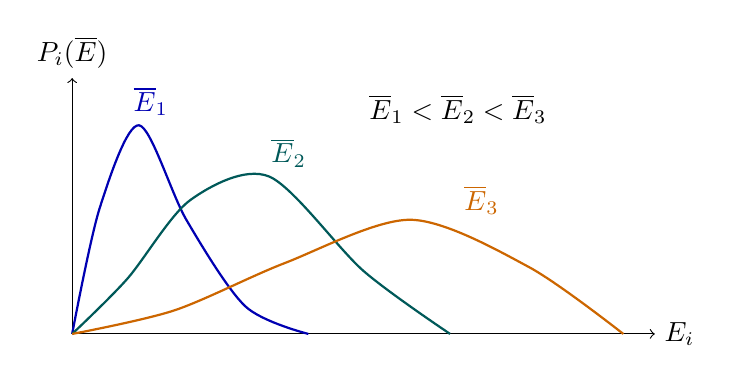
\begin{tikzpicture}[x=1cm,y=1cm]
\draw[->] (0,0) -- (7.4,0) node[right] {$E_i$};
\draw[->] (0,0) -- (0,3.25) node[above] {$P_i(\overline E)$};
\draw[thick,blue!70!black]
  plot[smooth] coordinates {(0,0) (0.35,1.6) (0.85,2.65) (1.45,1.45)
  (2.2,0.35) (3.0,0)};
\draw[thick,teal!70!black]
  plot[smooth] coordinates {(0,0) (0.7,0.7) (1.5,1.7) (2.5,2.0)
  (3.7,0.8) (4.8,0)};
\draw[thick,orange!80!black]
  plot[smooth] coordinates {(0,0) (1.3,0.3) (2.7,0.9) (4.3,1.45)
  (5.8,0.85) (7.0,0)};
\node[blue!70!black] at (1.0,2.95) {\(\overline E_1\)};
\node[teal!70!black] at (2.75,2.3) {\(\overline E_2\)};
\node[orange!80!black] at (5.2,1.7) {\(\overline E_3\)};
\node at (4.9,2.85) {\(\overline E_1<\overline E_2<\overline E_3\)};
\end{tikzpicture}
\caption{黒板のスケッチの清書版。曲線はこれらの正確な形を持つ必要はない。用いられているのは規格化と、それらの順序づけられた平均エネルギーのみである。}
\end{figure}

\begin{classroomqa}
\audiencequestion{この記法は循環しているのだろうか。平均エネルギーは分布から計算される一方、分布は平均エネルギーによってラベル付けされている。}
\lecturerresponse{経験的に選ばれた一パラメータ族の平衡分布から出発する。各成員は平均エネルギーをもつ。異なる成員が異なる平均をもつならば、その平均を族を名付けるパラメータとして用いることができる。この記法はまだ族を導出してはいない。ボルツマン分布がその導出を後にもたらすであろう。
\lecturetimestamp{00:28:35--00:29:44}}
\end{classroomqa}

\begin{classroomqa}
\audiencequestion{なぜ全エネルギーではなく平均エネルギーと言うのか。}
\lecturerresponse{部分系は、熱的に透過な壁をもつ気体容器の周囲の大気のような熱浴とエネルギーを交換している。その瞬間瞬間のエネルギーは揺らぐ。多数の測定は分布を生み出し、\(\overline E\) はそれらの結果の平均である。部分系と熱浴からなるより大きな閉じた系のエネルギーは依然として固定されていてもよい。
\lecturetimestamp{00:29:46--00:30:56}}
\end{classroomqa}

\begin{classroomqa}
\audiencequestion{異なる微視的状態が同じエネルギーをもつことはありうるか、また異なる分布が同じ平均エネルギーをもつことはありうるか。}
\lecturerresponse{どちらも可能である。平均エネルギーの制約だけでは多くの分布が許されるので、特別な一パラメータ平衡族には追加の物理的論証が必要である。その起源とそのボルツマン形は後で導出されるであろう。異なる微視的状態が等しいエネルギーをもつことは、縮退と呼ばれる別個の事柄である。
\lecturetimestamp{00:30:58--00:32:22}}
\end{classroomqa}

\subsection{状態ラベル、縮退、相関}

混同しやすいいくつかの区別を分離して保たなければならない。

第一に、多くの確率分布が同じ平均エネルギーをもちうる。一パラメータ平衡族は平均エネルギーの制約だけから得られるものではない。それは平衡化によって選ばれる特定の族であり、その形は後にボルツマン分布として同定されるであろう。

第二に、いくつかの異なる微視的状態が同じエネルギーをもちうる。これは縮退と呼ばれる。板書での議論では、状態をエネルギーによって曖昧さなく順序付けるために、厳密な縮退を一時的に無視する。縮退は実際、系が対称性をもつときにはよくあることだが、概念的問題を引き起こさない。状態ラベル \(i\) を保持し、\(E_i\) の値の重複を許し、すべての状態にわたって和をとればよい。

第三に、相関は縮退の別の言い方ではない。相関は二つの確率量の同時分布に関わり、一方を知ることが他方の確率を変えるかどうかを問う。一つの微視的状態のリストにおける互いに排他的なラベル \(i\) と \(j\) は、それ自体では、相関が計算されている二つの確率変数ではない。

\begin{classroomqa}
\audiencequestion{この構成は異なる \(i\) 状態が独立であると仮定しているのか、またそれらのうち二つが相関している場合はどうなるのか。}
\lecturerresponse{状態ラベルは一つの微視的確率変数の一つの可能な値である。独立性と相関には二つの同時分布する変数が必要なので、その用語はこのリストにおける二つの代替的なラベルに直接には当てはまらない。異なる状態が等しいエネルギーをもつことは、代わりに縮退に関する問題である。
\lecturetimestamp{00:32:23--00:33:22}}
\end{classroomqa}

\begin{classroomqa}
\audiencequestion{二つの異なる状態がまったく同じエネルギーをもつ場合はどうなるのか。}
\lecturerresponse{それは縮退である。当面のグラフのために、二つのエネルギーが一致しないという単純化の仮定を採用し、状態をエネルギーの増加順に並べる。後の確率の公式はこの仮定を必要としない。縮退した状態は単に別々に数えられるだけである。
\lecturetimestamp{00:33:23--00:34:04}}
\end{classroomqa}

\begin{classroomqa}
\audiencequestion{添字 \(i\) の意味は恣意的なのか。}
\lecturerresponse{微視的状態そのものは恣意的ではない。各状態は、厳密な記述に必要なすべての位置、運動量、その他のデータを指定する。それらの名前は恣意的なので、図のためにエネルギーが増加する順にラベルを選ぶ。
\lecturetimestamp{00:34:06--00:35:15}}
\end{classroomqa}

\section{エントロピーはエネルギーの関数となる}

平衡族の各成員はエントロピーをもつ。\eqref{eq:sm2-family} を \eqref{eq:sm2-equilibrium-entropy} に代入すると
\begin{equation}
 S(\overline E)
 =-\sum_iP_i(\overline E)\log P_i(\overline E).
 \label{eq:sm2-entropy-energy}
\end{equation}
が得られる。これはすべての物理系に共通する一つの普遍的な関数ではない。それは系のスペクトルとその平衡族に依存する。しかしひとたびその族が指定されれば、エネルギーとエントロピーは結びつけられる。族の中を動くことは両方を変化させる。

通常の系では、平均エネルギーが上昇するにつれて確率がより多くの状態に広がるのが典型的なので、\(S\) は通常 \(\overline E\) とともに上昇する。当面は、この関係が滑らかで局所的に可逆であると仮定する。例外は重要であるが、単純な場合が我々に必要な定義を明らかにする。

\section{温度を定義する導関数}

具体的な問いを立てよう。エントロピーを二進法の一つの選択肢分だけ増加させるには、平均エネルギーはどれだけ変化しなければならないか。自然対数の単位では、そのエントロピー増分は\(\log2\)である。

滑らかな族の隣接する要素に対して、
\begin{equation}
 dE=\frac{dE}{dS}\,dS.
 \label{eq:sm2-differential-identity}
\end{equation}
この時点では、この式は単なる連鎖律にすぎない。しかしその係数は、温度に要求される次元と物理的役割をまさに備えている。

\begin{definition}
エネルギー単位で表した温度は
\begin{equation}
 T\equiv\frac{dE}{dS}.
 \label{eq:sm2-temperature-definition}
\end{equation}
等価的に、
\begin{equation}
 dE=T\,dS,
 \qquad
 dS=\frac{1}{T}\,dE.
 \label{eq:sm2-fundamental-differentials}
\end{equation}
\end{definition}

1ビットの十分に小さな変化に対して、
\begin{equation}
 \Delta E\simeq T\log2.
 \label{eq:sm2-one-bit-energy}
\end{equation}
1ビットに固執するのは、導関数を具体的に実感するための方法にすぎない。任意の小さなエントロピー変化は同じ局所的な関係に従う。

\begin{classroomqa}
\audiencequestion{エントロピーが\(S(E)\)と書かれたのだから、\(dS/dE\)の方がより自然な導関数ではないだろうか。}
\lecturerresponse{関係が局所的に可逆であるとき、どちらの導関数も同じ情報を含んでいる：
\[
 \frac{dE}{dS}=\left(\frac{dS}{dE}\right)^{-1}.
\]
温度は慣例的に\(dE/dS\)であり、一方、逆温度は\(dS/dE=1/T\)である。
\lecturetimestamp{00:40:24--00:40:54}}
\end{classroomqa}

ここではただ一つの熱力学変数だけが変化しているので、通常の導関数で十分である。体積、粒子数、磁化、その他の変数が変化し得る場合には、偏導関数を用い、どの量を固定して保つかを明示しなければならない。現在の定義は、そのより一般的な熱力学幾何学の一変数断面である。

\subsection{なぜボルツマン定数が相殺されるのか}

温度計の単位に少し戻ろう。
\[
 T=k_{\mathrm B}T_{\mathrm K},
 \qquad
 S=\frac{S_{\mathrm C}}{k_{\mathrm B}},
\]
を用いると、基本関係は
\begin{align}
 dE
 &=\bigl(k_{\mathrm B}T_{\mathrm K}\bigr)
   d\left(\frac{S_{\mathrm C}}{k_{\mathrm B}}\right)\\
 &=T_{\mathrm K}\,dS_{\mathrm C}.
 \label{eq:sm2-carnot-form}
\end{align}
となる。\(k_{\mathrm B}\)の一方の因子は温度を通じて入り、逆数の因子はエントロピーを通じて入る。それらは相殺される。これが、従来の熱力学の教科書がボルツマン定数を表示せずに\eqref{eq:sm2-carnot-form}と書ける理由である。

\begin{classroomqa}
\audiencequestion{\(S(E)\)は可逆でなければならないか。}
\lecturerresponse{常にそうとは限らない。ここで考察する領域にある通常の系では、エネルギーを増加させると一般に平衡分布が広がりエントロピーが増大するので、\(S(E)\)は単調であり、\(T>0\)である。有界なスペクトルをもつ系は反例を与え得る。そこには、エントロピーがエネルギーとともに減少し、統計的温度が負になる領域も含まれる。それらの場合は今のところ脇に置く。
\lecturetimestamp{00:44:30--00:45:57}}
\end{classroomqa}

\section{抽象的な導関数から熱い・冷たいへ}

導関数による定義は普遍的だが、依然として抽象的である。我々は、エネルギーが熱い物体から冷たい物体へ流れるというおなじみの命題を回復したい。熱い表面に触れたときの痛みは生物学的なものであり、色や放出される放射は光の性質に依存する。統計的な定義は、放射を無視した場合でも、理想化された気体に対しても意味をなすべきである。

\begin{classroomqa}
\audiencequestion{熱い物体から放出される光が温度の基本的な定義を与え得るだろうか。}
\lecturerresponse{放射は有用な温度計であるが、光の物理学を持ち込んでしまう。統計力学は、気体の箱のような系に対しても、光学的性質に依拠せずに温度を定義しなければならない。エネルギーの交換の向きこそが、より一般的な判定基準である。
\lecturetimestamp{00:46:42--00:47:20}}
\end{classroomqa}

二つの系\(A\)と\(B\)を用意し、それぞれが最初はそれ自身の平衡にあり、温度は\(T_A\)と\(T_B\)であるとする。それらは最初、互いに孤立している。次に、それらを弱い熱接触を通じて接続する。すなわち、\emph{細い管}が、どちらの部分系の同一性も壊すことなく、少量のエネルギーを双方向に通過させる。

\begin{figure}[t]
\centering
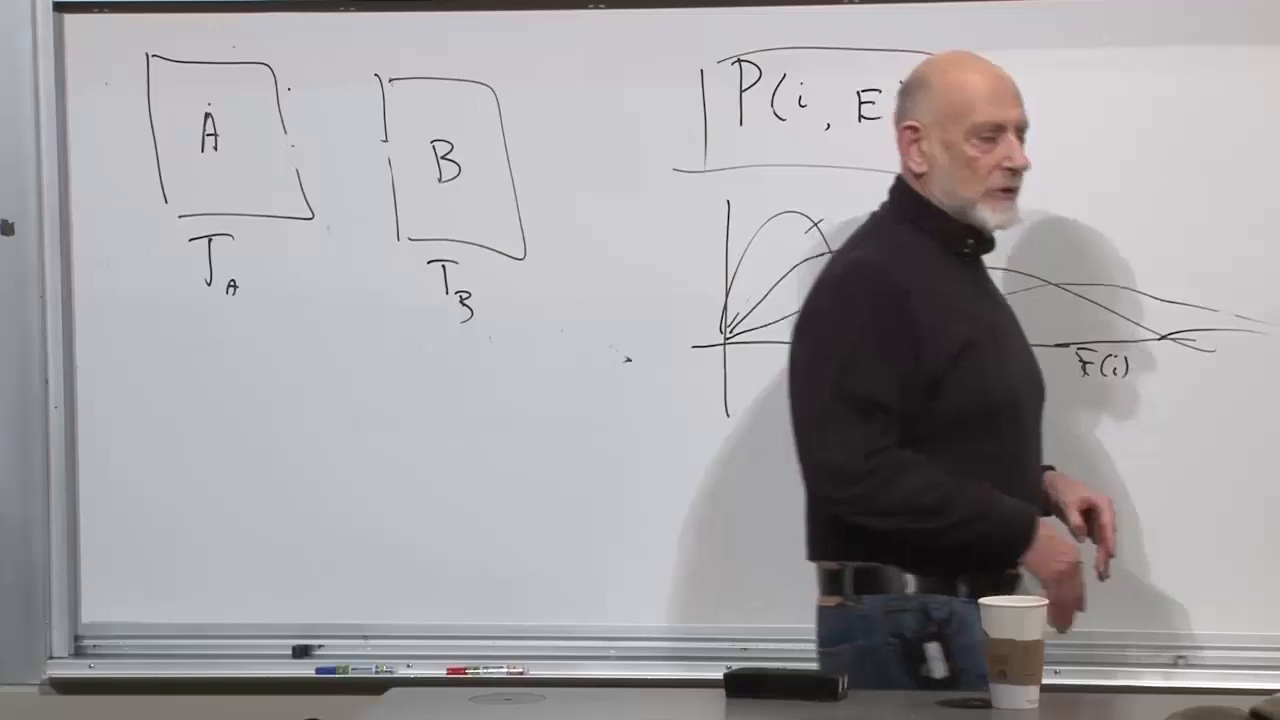
\includegraphics[width=0.88\textwidth]{lecture_02_figure_05.png}
\caption{別々に用意された系\(A\)と\(B\)は、温度\(T_A\)と\(T_B\)でラベル付けされ、弱い熱接触を考える直前の状態にある。}
\lectureframe{00:48:55}
\end{figure}

\begin{figure}[t]
\centering
\begin{tikzpicture}[>=Stealth]
\draw[rounded corners,thick,fill=blue!6] (0,0) rectangle (2.6,2.4);
\draw[rounded corners,thick,fill=orange!8] (5.4,0) rectangle (8,2.4);
\draw[thick] (2.6,1.35) -- (5.4,1.35);
\draw[thick] (2.6,1.05) -- (5.4,1.05);
\draw[<->,very thick] (3.15,1.2) -- (4.85,1.2)
  node[midway,above] {\(\delta E\)};
\node at (1.3,1.45) {\Large \(A\)};
\node at (6.7,1.45) {\Large \(B\)};
\node at (1.3,0.65) {\(T_A,S_A,E_A\)};
\node at (6.7,0.65) {\(T_B,S_B,E_B\)};
\node at (4,0.35) {\small weak thermal contact};
\end{tikzpicture}
\caption{複合系が孤立したままで、エネルギーが弱い接触を通じて揺らぐ。}
\end{figure}

一般性を失うことなく、
\begin{equation}
 T_B>T_A.
 \label{eq:sm2-temperature-order}
\end{equation}
と仮定する。経験によれば、\(B\)がエネルギーを失い、\(A\)がそれを得るはずである。三つの事実が、その予想を計算へと変える。

\subsection{エントロピーの加法性}

微視的な選択肢が独立に組み合わさる二つの弱く結合した部分系に対して、結合した可能性の数は掛け合わされる：
\[
 W_{AB}=W_AW_B.
\]
エントロピーは対数であるから、
\begin{equation}
 S_{\mathrm{tot}}=S_A+S_B.
 \label{eq:sm2-entropy-additivity}
\end{equation}
同じ結果は、積分布のシャノンエントロピーから直接導かれる。

\begin{classroomqa}
\classquestion{なぜ複合系のエントロピーは加算されるのか。}
\lecturerresponse{基礎となる選択肢の数が掛け合わされる一方で、エントロピーは対数をとるからである：
\(\log(W_AW_B)=\log W_A+\log W_B\)。弱い相互作用こそが、部分系の記述とこの主要な加法的形を可能にする。
\lecturetimestamp{00:51:06--00:52:03}}
\end{classroomqa}

\subsection{第一法則と第二法則}

合成系は孤立系であるから、内部で交換されるエネルギーは保存される：
\begin{equation}
 dE_A+dE_B=0,
 \qquad
 dE_B=-dE_A.
 \label{eq:sm2-first-law}
\end{equation}
これが本実験における第一法則である。

ここでは第二法則を公理として受け入れ、そのより深い説明は後に行う。
連結された系が新しい平衡へ緩和するとき、
\begin{equation}
 dS_{\mathrm{tot}}=dS_A+dS_B\geq0.
 \label{eq:sm2-second-law}
\end{equation}
厳密な不等号は平衡から離れた自発的緩和を表し、
等号は可逆な一次変分に対して平衡で成り立つ。

最後に、温度の定義は各々の部分系に適用される：
\begin{equation}
 dE_A=T_A\,dS_A,
 \qquad
 dE_B=T_B\,dS_B.
 \label{eq:sm2-two-temperatures}
\end{equation}

\begin{figure}[H]
\centering
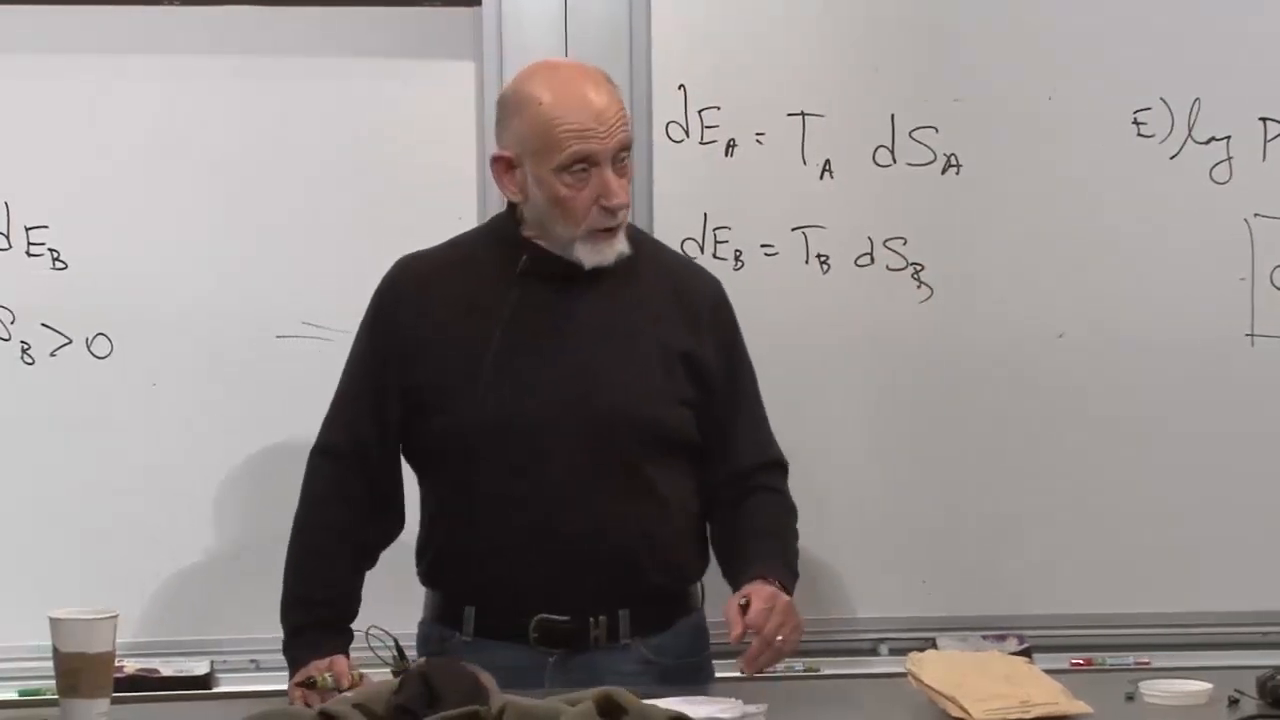
\includegraphics[width=0.88\textwidth]{lecture_02_figure_06.png}
\caption{黒板での議論の最後に現れた二つの部分系の関係
\(dE_A=T_A\,dS_A\) と \(dE_B=T_B\,dS_B\)。}
\lectureframe{00:54:00}
\end{figure}

\subsection{エネルギー流の符号}

これらの式はすでに正味の移動の向きを定めている。
\(dS_A=dE_A/T_A\)、\(dS_B=dE_B/T_B\)、および
\eqref{eq:sm2-first-law} を \eqref{eq:sm2-second-law} に代入すると：
\begin{align}
 dS_{\mathrm{tot}}
 &=\frac{dE_A}{T_A}+\frac{dE_B}{T_B}\\
 &=dE_A\left(\frac{1}{T_A}-\frac{1}{T_B}\right)\geq0.
 \label{eq:sm2-flow-sign}
\end{align}
もし \(T_B>T_A>0\) ならば、
\[
 \frac{1}{T_A}-\frac{1}{T_B}>0.
\]
したがって式 \eqref{eq:sm2-flow-sign} は
\[
 dE_A>0,
 \qquad
 dE_B<0.
\]
を要求する。
低温の系 \(A\) はエネルギーを得て、高温の系 \(B\) はそれを失う。
\(T_A=T_B\) のとき、一次のエントロピー変化は優先される向きを与えず、微視的な交換は釣り合って正味の流れはゼロになる。こうして、
抽象的な導関数 \(T=dE/dS\) は、高温と低温の操作的区別を再現する。
